\bilingualchapter{Forecasts}{预测值}

\begin{englishblock} WHAT DO THESE TERMS ALL HAVE IN COMMON: BREAKOUTS, Elliott waves, Fibonacci waves, exponentially weighted moving average crossover and Bollinger bands? Answer: They can all form the basis of trading rules. These rules give you forecasts of what they think will happen to the prices of instruments you are trading or investing in. Staunch systems traders use multiple systematic rules like these. But rules can also be extremely simple, like the single rule used by asset allocating investors. It's also possible to use my framework without any systematic rules at all, as a semi-automatic trader making your own discretionary forecasts. \end{englishblock}

\begin{chineseblock}这些术语有什么共同点：突破（breakouts）、艾略特波浪、斐波那契波浪、指数加权移动平均交叉以及布林带？答案是：它们都可以构成交易规则的基础。这些规则会给出预测，说明它们认为你正在交易或投资的品种价格接下来会怎么走。坚定的系统化交易者会使用多条这样的系统化规则。不过，规则也可以极其简单，比如资产配置型投资者所用的那条单一规则。甚至，你也完全可以不使用任何系统化规则，而是作为一名半自动交易者，在我的框架中直接使用你自己的主观预测。\end{chineseblock}

\bilingualsection{Chapter overview}{本章概览}

\begin{bilingualtableblock} \begin{tabularx}{\textwidth}{@{} L{0.30\textwidth} Y@{}}\textbf{What makes a good forecast} & Understand the important properties of the forecasts which trading rules produce. \\

\textbf{什么样的预测才算好} & 理解交易规则所生成预测值的重要性质。 \\
\textbf{Discretionary trading with stop losses} & How semi-automatic traders can make forecasts that have the right characteristics. \\
\textbf{带止损的主观交易} & 半自动交易者如何给出具有正确特征的预测值。 \\
\textbf{The asset allocating investor’s ‘no-rule’ rule} & The simplest possible trading rule used by asset allocating investors – a constant and identical forecast for all assets. \\
\textbf{资产配置型投资者的 “无规则”规则} & 资产配置型投资者所使用的最简单规则 ——对所有资产给出恒定且相同的预测。 \\
\textbf{Two systematic rules} & A pair of suggested trading rules for staunch system traders. \\
\textbf{两个系统化规则} & 为坚定的系统化交易者建议的一对交易规则。 \\
\textbf{Using other people’s rules} & How to adapt publicly available trading rules or invent your own. \\
\textbf{使用别人的规则} & 如何调整公开可见的交易规则，或自己发明规则。 \\
\textbf{Selecting trading rules and variation} & A brief reminder of how I recommend selecting rules and variations. \\
\textbf{选择交易规则与变体} & 我建议如何筛选规则及其变体的简要提醒。 \\
\end{tabularx}
\end{bilingualtableblock}

\bilingualsection{What makes a good forecast}{什么样的预测才算好}

\begin{englishblock} Parts of this section are quite technical; semi-automatic traders and asset allocating investors should read it but need only skim the content. However, staunch systems traders who will design their own trading rules need to understand it in detail. \end{englishblock}

\begin{chineseblock}本节中的部分内容相当技术化；半自动交易者和资产配置型投资者应当阅读，但只需浏览要点即可。然而，对于那些准备自己设计交易规则的坚定系统化交易者来说，这些内容则需要细致理解。\end{chineseblock}

\bilingualsubsection{A forecast is a scaled quantity}{预测值必须是一个有尺度的量}

\begin{englishblock} When I started trading options at a large investment bank I was encouraged to put on small proprietary positions outside of the normal customer flow trading. The idea was to give novices some practical experience in managing risk without exposing the book to large losses. Initially I was limited to trading single futures contracts. Once I graduated beyond one contract I was faced with a dilemma. How big should my position be for a purchase of German 10 year bond futures (Bunds)? Should I stick to one contract, or increase my size? I asked for advice from a more experienced trader, Sergei.\footnote{Not his real name. \par 这不是他的真名。} He sighed, exasperated at the ignorance of youth, and turned towards me. \end{englishblock}

\begin{chineseblock}当我刚开始在一家大型投资银行做期权交易时，我被鼓励在正常客户流交易之外，尝试建立一些小规模的自营头寸。这样做的目的，是让新手能获得一些实际风险管理经验，同时又不至于让交易账本暴露于过大的损失中。最初，我只能交易单份期货合约。当我终于被允许不止交易一份合约时，我遇到了一个难题。如果我想买入德国 10 年期国债期货（Bunds），那我的仓位到底应该有多大？我应该继续只做一份合约，还是可以加大规模？我去请教了一位更有经验的交易员，Sergei。他叹了口气，对年轻人的无知显得颇为无奈，然后转向我。\end{chineseblock}

\bipairgap

\begin{englishblock} "You need to know three things. First, how much do you like this trade? That comes from here," Sergei replied, pointing to his heart. "Second thing, how much can you afford to lose? That is down here, in your gut," and he patted his extensive stomach. "Last thing, how risky is it? You calculate that here." said Sergei, tapping his forehead. His answer was unhelpful, completely lacking in any detail, but totally correct. It's not enough to predict that prices are rising or falling; you also need to decide whether they will go up a lot, or a little. You need to decide how much you like the trade. You need a forecast -- a prediction of how much prices are expected to go up or down. This chapter is about making forecasts. I'll return to the rest of Sergei's wisdom in subsequent chapters. A forecast is a number: a positive value means you want to buy the asset because the price is expected to go up and a negative indicates you want to short the asset. Investors who don't use derivatives and can't short sell will only make positive forecasts. A forecast shouldn't be binary -- buy or sell -- but should be scaled. Forecasts close to zero indicate a small movement in prices and larger absolute values mean you expect bigger returns. There are three reasons why scaled forecasts make sense. Firstly, if you were to examine the returns made by a trading rule given the size of its forecasts, you'd normally find that forecasts closer to zero aren't as profitable as those further away. Secondly, binary systems cost more to trade, since to go from long to short you'd need to sell twice a full size position immediately. Finally, the rest of the framework assumes that the forecasts you get are not binary or lumpy in other ways.78 It's better to see forecasts changing continuously rather than jumping around. It's relatively easy to design or adapt a trading rule to produce scaled forecasts, if you're a staunch systems trader. If you're a semi-automatic trader generating forecasts in a more discretionary way then you need to be able to quantify the strength of your convictions and I'll return to that problem later in this chapter. Asset allocating investors have it easy since they use a fixed forecast value. \end{englishblock}

\begin{chineseblock}“你需要知道三件事。第一，你有多喜欢这笔交易？这个问题来自这里。”Sergei 一边说，一边指着自己的心脏。“第二件事，你最多能承受多大亏损？这个问题在这里，在你的肚子里。”说着他拍了拍自己宽大的肚皮。“最后一件事，这笔交易到底有多大风险？这个得用这里来算。”Sergei 一边说，一边敲了敲自己的额头。他的回答既不具体，也没有任何细节帮助，乍看之下几乎毫无用处，但实际上却完全正确。仅仅预测价格会上涨还是下跌还不够；你还需要判断它到底会涨很多，还是只涨一点。你必须决定自己到底有多看好这笔交易。你需要一个预测值--- 一个关于价格预期会涨或跌多少的预测。本章讲的就是如何构造这样的预测值。我会在后续章节中再回到 Sergei 的其余智慧上来。预测值本质上是一个数字：正值意味着你想买入该资产，因为你预期价格会上涨；负值则意味着你想做空该资产。那些不使用衍生品、也无法卖空的投资者，则只会有正的预测值。预测值不应当是二元的--- 不是简单地“买”或“卖”--- 而应当具有尺度。接近零的预测值表示价格只会小幅波动，而绝对值更大的预测值则表示你预期会有更大的收益。预测值必须带有尺度，背后有三个原因。第一，如果你去考察交易规则在不同预测值大小下产生的收益，通常会发现，接近零的预测值往往不如那些更远离零的预测值更赚钱。第二，二元系统的交易成本更高，因为当你从多头切换到空头时，你必须立刻卖出整整两倍的满仓头寸。第三，框架中的其余部分默认你得到的预测值不是二元的，也不会以其他方式呈现出离散跳跃的特征。78 让预测值连续变化，而不是一会儿跳来跳去，会更合理。对于坚定的系统化交易者来说，设计或改造一条能够输出连续尺度预测值的规则，其实并不难。而如果你是一个以更主观方式给出预测的半自动交易者，那么你就必须能够量化自己信念的强弱，这一点我会在本章后面再回来讨论。至于资产配置型投资者，他们就轻松多了，因为他们直接使用固定的预测值。\end{chineseblock}

\bilingualsubsection{Forecasts proportional to risk adjusted return}{预测值应当与风险调整后收益成比例}

\begin{englishblock} How do you set forecasts so that they embody how much you like a position, or to be precise how strong you think its subsequent rise or fall will be? \end{englishblock}

\begin{chineseblock}你该如何设定预测值，才能让它真正体现出你有多看好一个头寸，或者更准确地说，体现出你认为它接下来涨跌幅度会有多大？\end{chineseblock}

\begin{enumerate}
\item Technical notes: There are two main reasons for this. Firstly, forecasts should have well defined and relatively stable standard deviations, otherwise the risk properties of the trading system will not be well defined or stable. Secondly, as we'll see subsequently I recommend limiting absolute forecast values to twice their average. Forecast distributions which are more extreme than Gaussian normal distributions will see an undesirable level of forecast capping. Note that there is a special case where lumpy or even binary forecasts will work just fine. If we have a large number of relatively uncorrelated binary forecasts then once combined these will approach a desirable Gaussian normal. \end{enumerate}

\begin{enumerate}
\item 技术说明：这样做主要有两个原因。第一，预测值应当具有定义清晰且相对稳定的标准差，否则交易系统的风险特性就不会被清晰定义，也不会稳定。第二，正如我们稍后会看到的，我建议把预测值的绝对值限制在其平均值的两倍以内。如果预测值分布比高斯正态分布更极端，那么它们就会出现令人不希望的过度“封顶”现象。需要注意的是，也存在一种特殊情况，在这种情况下，带有跳跃性甚至完全二元的预测值也能很好地工作。如果我们拥有大量彼此相对不相关的二元预测值，那么它们在组合之后，也会逐渐逼近一种理想的高斯正态分布。\end{enumerate}

\begin{englishblock} Simple, you might think. As I was trading Bunds when I spoke to Sergei then I should set up my trading rule so a weak forecast of 50 would mean a purchase of 50 Bund futures. A strong forecast of 100 implies 100 contracts, and so on. Unfortunately there are several flaws in this idea. What if you wanted to use my forecasting rule? You might not want to take a gamble on even five Bunds, or you could work in a large fund for whom an average position would be 50,000 contracts. This kind of forecast doesn't account for different account sizes or varying appetite for risk. Secondly, what if the standard deviation of Bund prices were to double? A position of 50 contracts would now be twice as risky as you'd originally expected. The simple forecast doesn't account for risk changing over time. Finally, you'd normally want to use the same trading rule across different instruments, because it's simpler and it allows you to pool data if you're fitting. However 50 Bunds expose you to much less risk than 50 Japanese government ten year bond futures, but to much more than 50 German Schatz (two year) bond futures. The rule can't cope with instruments which don't have the same risk. The solution is to use my favourite technique, volatility standardisation. So in my framework forecasts are proportional to expected risk adjusted returns. For example suppose that the Bund has expected returns of 2\% a year and an expected annualised standard deviation of 8\%. Schatz futures have an expected return of 1\% a year, but you only expect volatility of 2\% a year. After adjusting for risk the expected return on Schatz (1\% ÷ 2\% = 0.5) is twice as much as on Bunds (2\% ÷ 8\% = 0.25). That implies the forecast for Schatz should be twice the forecast for Bunds. This deals with instruments that have different risks. It also means any trading rule can be used without modification on all instruments and that if you fit trading rules you can do so with pooled data from multiple assets. If you continuously adjust your estimate of expected volatility then you also cope with risk changing over time. Finally with forecasts like these different investors can use the same trading rules, but then scale positions depending on the size of their accounts and their appetite for risk. I show how this is done in chapter nine, ‘Volatility targeting', and chapter ten, ‘Position sizing'. You've seen before that the ratio of average return to standard deviation of returns is the Sharpe ratio. So expected Sharpe ratios make good forecasts, which makes creating trading rules very intuitive. \end{englishblock}

\begin{chineseblock}你可能会想，这很简单啊。既然我当时交易的是 Bund，那么我完全可以把交易规则设计成：弱预测值为 50 时，就买入 50 手 Bund 期货；而强预测值为 100 时，就买入 100 手，以此类推。可惜，这个想法有好几个漏洞。首先，如果是你想用我的预测规则呢？你也许连 5 手 Bund 都不愿意去赌；又或者你在一家大型基金工作，对你来说平均仓位可能是 50,000 手合约。这种预测方式无法考虑不同账户规模、也无法考虑不同风险偏好。其次，如果 Bund 的价格标准差突然翻倍怎么办？原本 50 手的仓位，现在风险就变成了你最初预期的两倍。这种简单预测并没有处理风险随时间变化的问题。最后，通常你会希望在不同品种之间使用同一条交易规则，因为这样更简单，也能让你在拟合时把多个资产的数据合并使用。然而，50 手 Bund 所暴露的风险，远低于 50 手日本十年期国债期货，却又远高于 50 手德国 Schatz（两年期国债）期货。这条规则无法应对风险水平不同的品种。解决方法，就是用我最喜欢的技术：波动率标准化。因此，在我的框架里，预测值与预期的风险调整后收益成正比。举个例子，假设 Bund 的预期年收益是 2\%，而预期年化标准差是 8\%。Schatz 期货的预期年收益是 1\%，但预期波动率只有 2\%。做完风险调整之后，Schatz 的预期收益（1\% ÷ 2\% = 0.5）就是 Bund （2\% ÷ 8\% = 0.25）的两倍。这意味着，Schatz 的预测值就应当是 Bund 的两倍。这样一来，就解决了不同品种风险不相同的问题。这也意味着，任何交易规则都可以不经修改地用在所有品种上；而如果你要拟合交易规则，也可以把多个资产的数据合并起来一起使用。如果你持续调整自己对预期波动率的估计，那么你也就能同时应对风险随时间变化的问题。最后，在这种预测值体系下，不同投资者完全可以使用同一套交易规则，只是在实际执行时，再根据账户规模和风险偏好去缩放仓位。我会在第九章“波动率目标”和第十章“仓位规模设定”中说明这是如何做到的。你之前已经见过，平均收益与收益标准差之比，就是夏普比率。因此，预期夏普比率天然就是一种很好的预测值表达方式，这也让交易规则的设计变得非常直观。\end{chineseblock}

\bilingualsubsection{Forecasts should have a consistent scale}{预测值应当具有一致的尺度}

\begin{englishblock} I said above that a forecast needs to be proportional to the risk adjusted return. In the example above forecasts of 2.5 for Bunds and 5 on Schatz; 0.0000005 and 0.000001 respectively, or 5,000 and 10,000, are all valid. Which of these, or the infinity of other options, is best? \end{englishblock}

\begin{chineseblock}我前面说过，预测值应当与风险调整后收益成正比。在刚才那个例子里，Bund 的预测值取 2.5，Schatz 取 5；或者分别取 0.0000005 和 0.000001；甚至取 5,000 和 10,000，其实都说得通。那么，在这些选择以及无限多其他可能性中，到底哪一种最好？\end{chineseblock}

\bipairgap

\begin{englishblock} In truth it doesn't really matter, as long as you are consistent, but whichever scaling you choose here will affect the rest of your trading system. In particular the expected average absolute value of your forecasts is a key part of specifying the system. Life will be easier if you choose a scaling that is easy to work with. Very small or large numbers are difficult for humans to cope with and even computers struggle with floating point representation of tiny fractions. My recommendation is to create forecasts which have an expected absolute value of 10. So +10 is an average buy and -10 an average sell. A forecast of +5 would be a weak buy, and -20 is a very strong sell. These forecast numbers may seem very abstract right now. Don't be too concerned as in chapter ten ‘Position Sizing' I will show you how to translate them into actual positions. If you're a semi-automatic trader using discretionary forecasts, it's straightforward to have the right scaling, as I will show you below. The rule used by asset allocating investors also has the appropriate scale. The example rules I provide for staunch systems traders later in the chapter are also correctly scaled. But if you're making your own rules, or adapting others, you will need to standardise their natural scaling, as I'll explain later in the chapter. \end{englishblock}

\begin{chineseblock}说实话，这件事本身并不重要，只要你始终保持一致即可。不过，无论你在这里选择什么样的尺度，它都会影响你交易系统的其他部分。尤其是，预测值的预期平均绝对值，是定义整个系统时的一个关键参数。如果你选用一个便于操作的尺度，后面的工作会轻松很多。过大或过小的数字，都不适合人类理解；而即便是计算机，在处理极小的小数浮点表示时也会遇到麻烦。我的建议是，把预测值设计成预期绝对值平均为 10。于是，+10 表示一个平均强度的买入，-10 表示一个平均强度的卖出。预测值 +5 表示一个偏弱的买入，而 -20 则表示一个非常强烈的卖出。这些预测值现在看起来也许很抽象，但不必太担心，因为我会在第十章“仓位规模设定”中告诉你，如何把它们转化为真实仓位。对于使用主观预测的半自动交易者而言，得到正确尺度其实很直接，下面我就会展示。资产配置型投资者所使用的那条规则，也天然拥有合适的尺度。我稍后在本章中给坚定系统化交易者提供的那些示例规则，也都已经被缩放到了正确尺度。但如果你打算自己设计规则，或者修改别人的规则，那么你就需要把它们原本的自然尺度重新标准化，正如我稍后会解释的那样。\end{chineseblock}

\bipairgap

\begin{englishblock} Should we allow forecasts to be as large as possible? With an expected absolute value of 10, a forecast of +10 is bullish, and one of +20 is really bullish. What if you're confident that this is the chance of a lifetime, like the 2009 Barclays trade which I told you about in the introduction. Should you allow your rule to have a forecast of +100? I think not. Forecasts should be capped at a maximum absolute value and I recommend a limit of 20. Here's why: \end{englishblock}

\begin{chineseblock}我们是否应该允许预测值无限增大？如果预期绝对值平均为 10，那么预测值 +10 表示看多，而 +20 则表示非常看多。但如果你坚信这是一生一次的机会，比如我在导言里讲到的 2009 年巴克莱交易，你是否就应该允许规则给出 +100 这样的预测值？我认为不应该。预测值应当设定一个绝对值上限，而我建议这个上限设为 20。原因如下：\end{chineseblock}

\bipairgap

\begin{englishblock} Risk control Diversification is the investor's best friend. But it's pointless diversifying if you then allow one part of your system to dominate your returns. You need to limit the risk that any trading rule variation can contribute to the overall system. \end{englishblock}

\begin{chineseblock}风险控制 分散化是投资者最好的朋友。但如果你一边做分散化，一边却允许系统中的某个部分支配你的整体收益，那么分散化就失去了意义。你必须限制任何单一交易规则变体对整个系统所能贡献的风险。\end{chineseblock}

\bipairgap

\begin{englishblock} Limited data When I back-test a profitable trading rule I normally find that positive forecasts are associated with price rises, and larger values mean larger rises. However for a properly scaled rule very large forecast values will appear rarely in a back-test. So there is a lot of uncertainty around whether extremely large forecasts translate into proportionally larger price movements, as I don't usually have enough data to support this finding. If a forecast had a Gaussian normal distribution you'd only see absolute forecast values over 20 around 5\% of the time, so there is only limited evidence that forecasts of this magnitude are actually correct. \end{englishblock}

\begin{chineseblock}数据有限 当我回测一条有盈利能力的交易规则时，通常会发现：正的预测值往往伴随着价格上涨，而且预测值越大，上涨幅度通常也越大。然而，对于一条已经正确缩放过的规则来说，特别大的预测值在回测中其实很少出现。因此，我们并没有足够多的数据去支持这样一个结论：极端大的预测值是否真的对应按比例更大的价格波动。如果预测值服从高斯正态分布，那么绝对值超过 20 的情况只会在大约 5\% 的时间里出现，所以我们对于这种量级预测值的正确性，实际上只有非常有限的证据。\end{chineseblock}

\bipairgap

\begin{englishblock} Extremes are Normally markets trend with falls followed by further falls, but after very often different sharp drops subsequent one day rises are more likely; the so called ‘dead cat bounce'. Similarly high yielding stocks do well, but those with dividend yields above 50\% are probably going bankrupt, or at the very least about to cut their dividend. Many other patterns also reverse at extremes. These effects are not often strong or common enough to exploit directly, but they should give you concern about betting too much when you have very strong forecasts. \end{englishblock}

\begin{chineseblock}极端值经常并不一样 一般来说，市场下跌之后往往会继续下跌，但在某些非常剧烈的暴跌之后，次日上涨的概率反而更大，这就是所谓的“死猫反弹”。类似地，高股息率股票通常表现不错，但那些股息率高到超过 50\% 的股票，很可能已经快要破产，至少也很可能马上要削减分红。很多其他模式，在极端位置时也会反转。虽然这些效应往往既不够强也不够常见，不足以被直接拿来利用，但它们至少应当提醒你：当预测值非常强时，你不该贸然下过重的赌注。\end{chineseblock}

\bipairgap

\begin{englishblock} Higher realised A high forecast could mean that you expect large returns, but equally return volatility might be due to very low standard deviation of returns. Unfortunately periods of subdued volatility are usually followed by jumps to much higher levels, often combined with reversals in price. I had very strong positive forecasts in the Japanese Bond markets in January 2013, mainly due to relatively low volatility. When Prime Minister Abe unveiled his latest set of economic reforms volatility spiked rapidly as prices dropped fast. Fortunately because my forecasts were capped the damage was contained. \end{englishblock}

\begin{chineseblock}更高的实际收益波动 高预测值可能意味着你预期会有很大收益，但它同样也可能只是因为收益标准差暂时特别低。遗憾的是，低波动时期之后往往会突然出现更高波动，而且这种波动上升常常伴随着价格反转。2013 年 1 月，我在日本债券市场上就曾出现过很强的正向预测值，而主要原因正是当时波动率比较低。后来安倍首相公布了一套新的经济改革方案，波动率迅速飙升，价格也快速下跌。幸运的是，由于我的预测值早已设置了上限，所以损失被控制住了。\end{chineseblock}

\bipairgap

\begin{englishblock} Limited If forecasts have a Gaussian normal distribution then it's rare, again around downside 5\% of the time, that you'll see values bigger than 20. So the reduction in your returns from capping is quite small compared to the potential risk control benefits. \end{englishblock}

\begin{chineseblock}下行代价有限 如果预测值服从高斯正态分布，那么超过 20 的情况本来就很少见，大约只占 5\% 的时间。因此，相比于它所带来的风险控制好处，把预测值封顶对收益的拖累其实是很小的。\end{chineseblock}

\bipairgap

\begin{englishblock} Staunch systems traders shouldn't ignore forecasts that are outside of the range -20 to +20, but cap them. A forecast of +25 from your trading rule should be reduced to +20. Increase any forecast lower than -20 to that level. All your forecasts will then be in the range -20 to +20. For semi-automatic traders all your discretionary forecasts should be in the range of -20 to +20, with no exceptions, even for the trade of a lifetime. Asset allocating investors don't need to worry as you will have a fixed forecast of +10. If we can't short an instrument, because of limited access to derivatives or difficulties selling short, then you'll also need to change all negative forecasts to zero. \end{englishblock}

\begin{chineseblock}坚定的系统化交易者不应该无视超出 -20 到 +20 区间的预测值，而应当把它们封顶。例如，一条交易规则给出 +25 的预测值时，你应把它压到 +20；任何低于 -20 的预测值，也都应抬升到 -20。这样，你的所有预测值就都被限制在 -20 到 +20 之间。对于半自动交易者来说，你的所有主观预测值也都应严格限制在 -20 到 +20 之间，没有任何例外，哪怕你觉得自己正面对一生一次的交易机会也是如此。资产配置型投资者则不必担心这一点，因为你的预测值固定为 +10。如果我们无法做空某个品种，可能是因为无法获得足够的衍生品工具，或者卖空存在困难，那么你还需要把所有负预测值都改为 0。 \end{chineseblock}

\bilingualsection{Discretionary trading with stop losses}{带止损的主观交易}

\bilingualsubsection{Semi-automatic Trader}{半自动交易者}

\begin{englishblock} If you're a semi-automatic trader then you won't use systematic trading rules but instead make discretionary forecasts either on gut feeling, or using complex analysis which can't be systematised, like my 2009 Barclays trade in the introduction. As well as the sign of the forecast, positive for long and negative for short, you must indicate how strongly you feel about it. Your forecasts must be correctly scaled: the expected absolute value should be around 10, and they must be between the recommended limits of -20 and +20. Forecasts don't have to be finely quantified, such as "I love the Nikkei today, about 8.7663." However, you should be able to give a rough indication of the strength of your passion for the Nikkei. You can then translate your opinion into a forecast number, as table 16 shows. \end{englishblock}

\begin{chineseblock}如果你是半自动交易者，那么你不会使用系统化交易规则，而是会依据直觉，或者依据那些无法系统化的复杂分析来给出主观预测，就像我在导言中讲到的 2009 年那笔巴克莱交易一样。除了预测值的方向之外--- 做多时为正，做空时为负--- 你还必须说明自己对这个判断到底有多强的信心。你的预测值必须被正确缩放：预期绝对值平均应大约为 10，并且必须落在建议区间 -20 到 +20 之间。预测值不需要被精确量化成类似“我今天特别看好日经指数，大概是 8.7663”这种程度。但你至少应当能够大致表达，你对日经指数的热爱究竟有多强。然后，你就可以像表 16 所展示的那样，把自己的判断翻译成一个预测值数字。\end{chineseblock}

\begin{chinesetableblock} \rawtablecaption{TRANSLATING OPINIONS INTO A QUANTIFIED FORECAST\\把主观判断转换为量化预测值}\begingroup \small \setlength{\tabcolsep}{2pt} \renewcommand{\arraystretch}{1.15} \noindent\begin{tabularx}{\textwidth}{@{}*{9}{>{\centering\arraybackslash} X}@{}}\toprule \shortstack{Very\\strong\\sell} & \shortstack{Strong\\sell} & Sell & \shortstack{Weak\\sell} & Neutral & \shortstack{Weak\\buy} & Buy & \shortstack{Strong\\buy} & \shortstack{Very\\strong\\buy} \\
\midrule
-20 & -15 & -10 & -5 & 0 & 5 & 10 & 15 & 20 \\
\bottomrule
\end{tabularx}
\endgroup \end{chinesetableblock}

\begin{chinesetableblock} \begingroup \small \setlength{\tabcolsep}{2pt} \renewcommand{\arraystretch}{1.15} \noindent\begin{tabularx}{\textwidth}{@{}*{9}{>{\centering\arraybackslash} X}@{}}\toprule \shortstack{非常\\强烈\\卖出} & \shortstack{强烈\\卖出} & 卖出 & \shortstack{偏弱\\卖出} & 中性 & \shortstack{偏弱\\买入} & 买入 & \shortstack{强烈\\买入} & \shortstack{非常\\强烈\\买入} \\
\midrule
-20 & -15 & -10 & -5 & 0 & 5 & 10 & 15 & 20 \\
\bottomrule
\end{tabularx}
\endgroup \end{chinesetableblock}

\begin{englishblock} If you can’t go short assets, because you’re not using derivatives like spread bets or can’t short sell in your account, then you’ll need to limit yourself to positive forecast values. You shouldn’t change your forecast once a bet is open. Otherwise there is the risk of meddling, taking profits too early by reducing the conviction of your forecast or doubling up on a loss. Instead you will be using a systematic trailing stop loss rule to close all your positions. I’ll explain this further in chapter thirteen, where I describe a semi-automatic trading system in more detail. There are substantial advantages to using discretionary forecasts in my systematic framework with stop losses; you can make predictions about the behaviour of your live trading and measure expected risk more precisely. Your positions will always be the correct size for a given forecast, tolerance for risk, and account size. This will give you more time and energy to get the forecast right. Finally, by using stop losses you’ll be trading somewhat like an ‘early loss taking’ trend follower, so it’s more likely your strategy will have benign positive skew. \end{englishblock}

\begin{chineseblock}如果你不能做空资产，可能是因为你没有使用点差投注之类的衍生品，或者你的账户本身不允许卖空，那么你就必须把自己限制在只使用正的预测值。一旦某笔下注已经建立，你就不应该再去修改自己的预测值。否则，你就会面临“干预”的风险：比如因为降低自己对预测的信心而过早止盈，或者因为亏损而不断加码。相反，你应该使用系统化的跟踪止损规则来关闭所有头寸。我会在第十三章里更详细地说明这一点，那里我会完整描述一套半自动交易系统。在我的系统化框架中，把主观预测与止损结合起来，会带来非常明显的优势：你可以更精确地预测自己实盘交易的行为特征，也能更准确地衡量预期风险。你的仓位始终会根据给定的预测值、风险承受能力和账户规模而保持正确大小。这样一来，你就能把更多时间和精力放在如何把预测做对上。最后，由于你会使用止损，你的交易行为会在某种程度上更像一个“尽早止损”的趋势跟随者，因此你的策略更有可能呈现出较为温和的正偏度。\end{chineseblock}

\bilingualsection{The asset allocating investor’s ‘no-rule’ rule}{资产配置型投资者的“无规则”规则}

\bilingualsubsection{Asset Allocating Investor}{资产配置型投资者}

\begin{englishblock} Think about a static portfolio of two collective funds: an S\&P 500 equity and a US benchmark bond fund. Suppose you bought them in equal weights, with half your cash in each. As bond funds tend to have a quarter of the volatility of equities this portfolio will have 80\% of its risk coming from stocks. As I explained in chapter two the solution is to hold the two assets in risk parity, each contributing the same amount of expected risk. This implies a cash weight to equities of roughly 20\% and 80\% to bonds. By using the framework, instruments will automatically have identical expected standard deviation of returns for a given forecast level. This means if you have an equally weighted portfolio of two trading subsystems, one for equities and one for bonds, each with identical forecasts for their individual instrument, then you'd always have the same expected volatility for both equities and bonds. You'd effectively have a risk parity strategy where risk was being constantly adjusted, or what I described in chapter two as a ‘fourth degree' static portfolio (page 38). Hence the correct rule for an asset allocating investor is to have a constant forecast equal to the expected average forecast, +10 for all instruments at all times. I call this the ‘no-rule' rule. You don't think you can predict how different assets will perform, so you buy them all. Remember all forecasts are proportional to return adjusted for standard deviation. So using an equal forecast for all instruments is equivalent to assuming all assets have the same expected Sharpe ratio. There are certain advantages to using this constant forecast approach within the systematic framework, rather than just buying a normal risk parity portfolio. For starters you can probably do better than equal weights, as you will remember from chapter four, ‘Portfolio allocation'. Secondly, many risk parity funds don't adjust for the standard deviation of returns changing over time, whereas you will.79 As I'll discuss in chapter twelve, ‘Speed and Size', that adjustment will be done after carefully considering the trading costs of our instruments. A DIY risk parity portfolio avoids paying the management fees you'd have with an external fund manager. Finally, if you do decide to introduce expectations of asset returns there is a neat and relatively robust way to do this, by adjusting handcrafted portfolio weights in line with where you think prices will go. I'll give you more detail in the asset allocating investor example in part four of the book. \end{englishblock}

\begin{chineseblock}想象一个由两个集合基金组成的静态组合：一个 S\&P 500 股票基金和一个美国基准债券基金。假设你以相等现金权重买入它们，也就是各投入一半现金。由于债券基金的波动率通常只有股票基金的大约四分之一，这样的组合其实会有 80\% 的风险来自股票。正如我在第二章中解释过的，解决方法是让这两个资产处于风险平价状态，也就是各自贡献相同数量的预期风险。这意味着，股票大约只应占 20\% 的现金权重，而债券则应占 80\%。通过使用这个框架，对于给定的预测值水平，不同品种将自动拥有相同的预期收益标准差。这意味着，如果你拥有一个由两个交易子系统组成、且现金权重相同的投资组合，其中一个负责股票，另一个负责债券，并且它们都对各自品种使用相同的预测值，那么股票和债券将始终具有相同的预期波动率。实际上，你就得到了一种会持续调整风险的风险平价策略，也就是我在第二章中称作“四度静态组合”的东西（第 38 页）。因此，对于资产配置型投资者来说，正确的规则就是：对所有品种，在所有时间点上都使用一个恒定预测值，这个预测值等于预期平均预测值，也就是 +10。我把它称为“无规则”规则。你并不认为自己能够预测不同资产的相对表现，所以你就把它们都买进来。请记住，所有预测值本质上都与标准差调整后的收益成正比。因此，对所有品种使用相同预测值，就等价于假设所有资产都拥有相同的预期夏普比率。与其直接买入一个普通的风险平价投资组合，在这个系统化框架中使用恒定预测值，其实还有一些额外优势。首先，正如你在第四章“投资组合配置”中会记得的那样，你大概率可以做得比简单等权更好。其次，许多风险平价基金并不会根据收益标准差随时间的变化来动态调整，而你会。79 正如我会在第十二章“速度与规模”中讨论的那样，这种调整会在仔细考虑交易成本之后进行。自己动手做一个风险平价组合，也可以避免向外部基金经理支付管理费。最后，如果你确实决定引入对资产收益的主观预期，那么还有一种相当整洁且相对稳健的方式来实现这一点：你只需根据自己认为价格会如何变化，相应调整手工构造的投资组合权重即可。我会在本书第四部分的资产配置型投资者示例中，给你更多细节。\end{chineseblock}

\bilingualsection{Two example systematic rules}{两个示例系统化规则}

\bilingualsubsection{Staunch Systems Trader}{坚定的系统化交易者}

\begin{englishblock} Semi-automatic traders and asset allocating investors can skip the remainder of this chapter, which is for staunch systems traders only. The two examples of trading rules above aren't very interesting. I include them to show how my framework can still be used by people who don't believe that market returns can be forecasted, or others who think they can do it better than a simple rule can. However staunch systematic traders disagree with both of these groups and wish to forecast prices with fully systematic trading rules. There isn't enough space in this book to include every trading rule in existence. Fortunately, there's a plethora of other books and websites available which contain explicit trading rules, or ideas from which they can be developed. Just one book, Perry Kaufman's Trading Systems and Methods has over 1000 pages and includes dozens of rules.80 The next section in this chapter will show how you can create your own trading rules, or modify other people's. In this section I will briefly outline two rules that I use in my own trading system.81 If you want to use them you can find more detail in appendix B. In part four of this book I'll show how these rules can be incorporated into the framework to create a complete system for the staunch systems trader. \end{englishblock}

\begin{chineseblock}半自动交易者和资产配置型投资者可以跳过本章余下的内容，因为下面的部分只写给坚定的系统化交易者。上面那两个交易规则示例其实并不算有趣。我之所以仍然把它们写进来，是为了说明：即便对于那些不相信市场收益可以被预测的人，或者那些相信自己能比简单规则做得更好的人，我的框架依然是可用的。不过，坚定的系统化交易者与这两类人都不同，他们希望通过完全系统化的交易规则来预测价格。本书没有足够篇幅把世上所有交易规则都列出来。幸运的是，市场上已经有大量书籍和网站，里面要么直接给出了明确规则，要么至少提供了可供开发的思路。仅仅 Perry Kaufman 的\textit{Trading Systems and Methods} 一书就超过 1000 页，包含了几十条规则。80本章下一节会展示，如何创建你自己的交易规则，或者如何修改别人的规则。而在这一节里，我会简要介绍两条我自己在交易系统中所使用的规则。81如果你想真正使用它们，可以在附录 B 中找到更详细的说明。到了本书第四部分，我还会展示如何把这些规则纳入框架，构建出一套完整的坚定系统化交易者系统。\end{chineseblock}

\bilingualsubsection{Trend following with the EWMAC rule}{使用 EWMAC 规则进行趋势跟踪}

\begin{englishblock} Many asset prices seem to show momentum: what goes up, usually carries on going up; and vice versa. This effect can be captured by using trend following rules. I am a big fan of these types of rules for several reasons. Firstly, they work. As we saw in chapter one, the trend following ‘early loss taker' rule made mincemeat of its opposition, the ‘early profit taker'. There's a lot of academic research and real performance statistics supporting the use of trend following rules. Secondly, I like rules which I can explain; as I said in chapter two prospect theory justifies why these rules work, and should continue to do so. Also, trend following is an easy to implement technical strategy using only price data. Finally, it has benign positive skew. \end{englishblock}

\begin{chineseblock}许多资产价格似乎都存在动量效应：上涨的东西通常会继续上涨，反之亦然。趋势跟踪规则正是用来捕捉这一效应的。我非常喜欢这类规则，原因有好几个。首先，它们确实有效。正如我们在第一章中看到的那样，趋势跟踪式的“尽早止损者”规则，把它的对手“尽早止盈者”打得体无完肤。大量学术研究以及真实表现统计都支持趋势跟踪规则的有效性。其次，我喜欢那些我能够解释清楚的规则；正如我在第二章中所说，前景理论能够解释这些规则为什么有效，以及为什么它们应该继续有效。此外，趋势跟踪还是一种非常容易实现的技术型策略，因为它只需要价格数据即可。最后，它还具有相对温和的正偏度。\end{chineseblock}

\bipairgap

\begin{englishblock} Of course you could use the now familiar early loss taker rule for trend following, but there are better alternatives.82 One of the most popular trading rules for capturing trends goes by the unwieldy name of Exponentially Weighted Moving Average Crossover, or EWMAC for short.\footnote{This is probably one of the oldest purely systematic trading rules in current use; ignoring the older, more subjective, technical analysis pattern matching tradition. There are academic studies of EWMAC dating back to the 1960s and it would have been used by traders prior to that. \par 这可能是目前仍在使用的最古老的纯系统化交易规则之一（如果不算更早、更主观的技术分析图形识别传统的话）。有关 EWMAC 的学术研究可以追溯到 20 世纪 60 年代，而在那之前，交易者实际上就已经在使用类似方法了。} Fortunately the idea is simpler to implement than it is to say. You take two exponentially weighted moving averages (EWMA) of an asset's price. One average, the slower, looks back over a longer period than the faster average. When the faster is above the slower it means that prices are in an uptrend and you should buy; and vice versa. \end{englishblock}

\begin{chineseblock}当然，你也完全可以用现在已经很熟悉的“尽早止损者”规则来做趋势跟踪，但其实还有更好的替代方案。82在捕捉趋势方面，最流行的规则之一有一个很拗口的名字：指数加权移动平均交叉（Exponentially Weighted Moving Average Crossover），简称 EWMAC。幸运的是，这个想法真正实现起来，比把它说出来要简单得多。你只需要对某个资产的价格计算两条指数加权移动平均线（EWMA）。其中一条均线回看期更长，叫慢均线；另一条回看期更短，叫快均线。当快均线位于慢均线之上时，就说明价格处于上升趋势，此时你应当买入；反之亦然。\end{chineseblock}

\begin{figure}[htbp] \centering 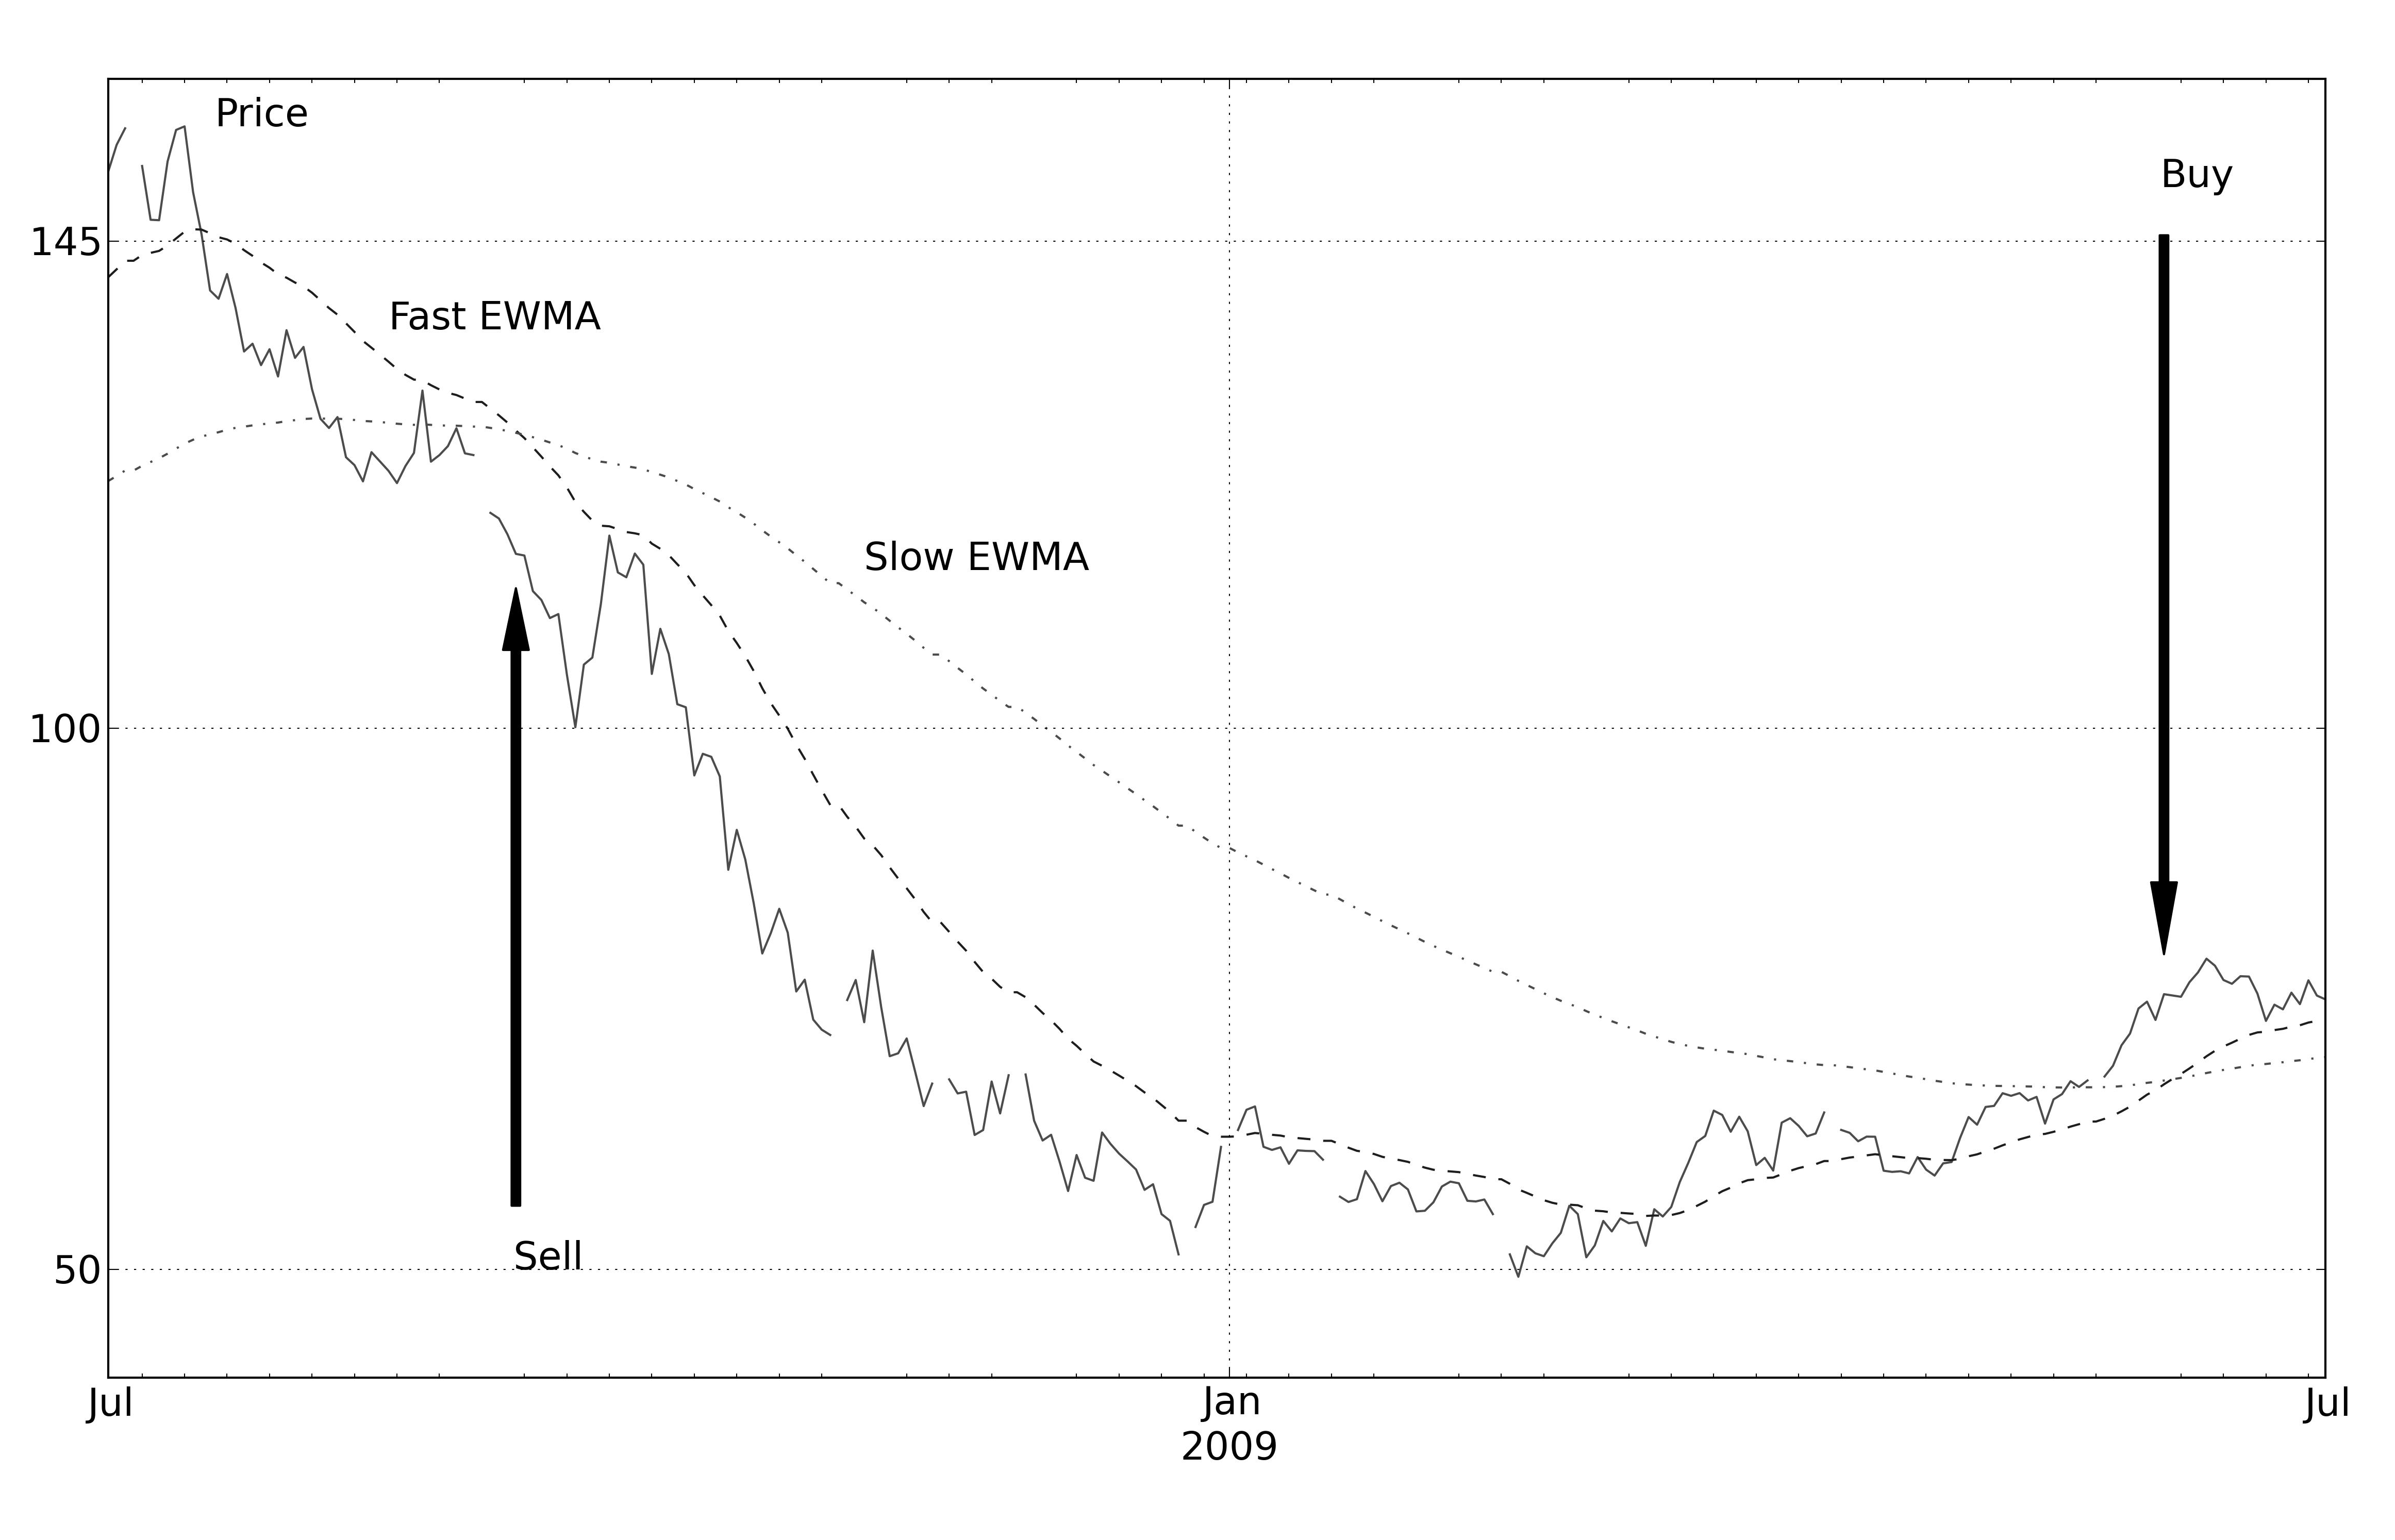
\includegraphics[width=\textwidth]{figures/raw/img-018.png} \caption{RIDING THE DOWNTREND IN CRUDE OIL FUTURES WITH THE EWMAC TREND FOLLOWING RULE. WE SELL WHEN THE FAST EWMA CROSSES THE SLOW; AND BUY WHEN THIS REVERSES\\
使用 EWMAC 趋势跟踪规则顺势做空原油期货的下跌行情。当快 EWMA 下穿慢 EWMA 时我们卖出；当这一关系反转时我们买入}\end{figure}

\begin{englishblock} Figure 18 shows an example. Here we've got the price of crude oil futures from summer 2008 onwards. After a long uptrend in prices there is a reversal in July 2008. Within a few weeks the fast EWMA has gone below the slower and goes short. The gap gets bigger and the position is increased until January. A gentle bullish trend begins and the short \end{englishblock}

\begin{chineseblock}图 18 展示了一个例子。这里我们看到的是从 2008 年夏天开始的原油期货价格。在经历了一段长时间的上涨趋势之后，价格在 2008 年 7 月发生了反转。几周之内，快 EWMA 就跌破了慢 EWMA，于是系统转为空头。两条均线之间的差距不断扩大，因此仓位会持续增加，一直到次年一月。随后，一段温和的上涨趋势开始出现，而空头仓位\end{chineseblock}

\begin{enumerate}
\item Early loss taker has some unpleasant attributes. First of all it gives a binary forecast; you are either long or short. Secondly, your current forecast depends on prices but also what positions you have recently had. This isn't a very nice property; amongst other things it means your precise back-tested behaviour will depend on where your price history began. \end{enumerate}

\begin{enumerate}
\item “尽早止损者”规则有一些不太讨喜的特征。首先，它给出的是二元预测值；你要么做多，要么做空。其次，你当前的预测值不仅依赖价格，还依赖你最近持有什么仓位。这并不是一种很理想的性质；其中一个问题是，它会导致你的精确回测行为取决于价格历史从哪里开始。\end{enumerate}

\begin{englishblock} is reduced, and then reversed once the fast EWMA climbs back above the slow in June \end{englishblock}

\begin{chineseblock}便开始逐步减小，直到 6 月快 EWMA 再次上穿慢均线之后，仓位才真正反向。\end{chineseblock}

\begin{enumerate}
\item There is a detailed specification of the EWMAC rule in appendix B. \end{enumerate}

\begin{enumerate}
\item 附录 B 中给出了 EWMAC 规则的详细定义。\end{enumerate}

\bilingualsubsection{The carry rule}{Carry 规则}

\begin{englishblock} EWMAC is a positive skew rule which needs prices to trend in one direction or another. To balance it out here is the carry rule which benefits when nothing happens. Foreign exchange carry is a well known strategy for exploiting stable markets; if you borrow in Japanese yen at 0.5\% and invest the money in Australian dollars at 3.5\% then you'll earn 3\%, assuming that the JPY/AUD exchange rate doesn't budge. But what does carry mean for other assets?\footnote{The first multi asset (rather than FX specific) academic research into carry appears to be the imaginatively titled working paper ‘Carry' by Ralph Koijen, Tobias Moskowitz, Lasse Pedersen and Evert Vrugt from 2012. The specification of the carry rule here is identical to that paper. But rules like this have been used in the industry for much longer. \par 第一篇关于多资产（而非仅限外汇）的 carry 学术研究，似乎是 Ralph Koijen、Tobias Moskowitz、Lasse Pedersen 和 Evert Vrugt 在 2012 年发表的工作论文《Carry》。这里给出的 carry 规则定义与那篇论文一致。但类似的规则在行业中被使用的时间其实要长得多。} Carry, which is sometimes called roll down or contango, is the return that you will get if asset prices are perfectly stable. If the world doesn't change this will be equal to the yield on the asset, less the cost of borrowing (or the interest you would have got from holding cash). So if you buy shares in French supermarket Carrefour which currently has a dividend yield of 3\%, and you pay 1\% to borrow the purchase cost, then you earn 2\% carry on the position if the share price is unchanged. Similarly today I can buy June 2018 Eurodollar futures at 97.94, or March 2018 at 98.01. If there is no change in the shape of the yield curve then in three months' time June futures will rise to 98.01, earning 0.07 per contract. Academic theory predicts that prices should move against us to offset these returns, but it often doesn't. Carry is usually earned steadily on these kinds of trades although occasionally they go horribly wrong and the relationship temporarily breaks down, giving this trading rule some evil negative skew. I think the rule is profitable as a reward for taking on this nasty skew and various other kinds of risk premium which tend to be correlated to carry trades. Full details on how I calculate carry are given in appendix B, from page 285 onwards. There is an example of the carry trading rule in action in figure 19, again showing crude oil futures during the great crash of 2008. The price of the nearer futures contract dips below the contract we are trading in mid-August. This is a bearish carry signal and the rule sells to enjoy some of the continuing fall in price. \end{englishblock}

\begin{chineseblock} EWMAC 是一条正偏度规则，它需要价格朝某个方向形成趋势。为了与之平衡，我再介绍另一条在“什么都没发生”时也能赚钱的规则：carry 规则。外汇 carry 是一种很著名的稳定市场套利策略：如果你以 0.5\% 的利率借入日元，然后把钱投资到利率为 3.5\% 的澳元资产中，那么只要 JPY/AUD 汇率不发生变化，你就能赚到 3\% 的收益。但 carry 在其他资产上又意味着什么呢？Carry 有时也被称为 roll down 或 contango，它指的是：如果资产价格完全保持不变，你能够从中获得的那部分收益。如果世界没有变化，那么这个收益就等于该资产本身的收益率，减去融资成本（或者减去你持有现金本来可以拿到的利息）。例如，如果你买入法国超市 Carrefour 的股票，而它当前股息率是 3\%，同时你为了购买它而支付 1\% 的融资成本，那么只要股价不变，你在这个头寸上的 carry 收益就是 2\%。同样地，如果今天我以 97.94 的价格买入 2018 年 6 月到期的欧元美元期货，或者以 98.01 的价格买入 2018 年 3 月到期的合约，那么只要收益率曲线的形状不变，三个月之后，6 月合约的价格就会上升到 98.01，从而为我每份合约赚到 0.07 的收益。学术理论会预测，价格应该朝不利于我们的方向移动，以抵消这些收益，但现实中它往往并不会这样。Carry 规则通常会在这类交易中稳定赚钱，尽管偶尔它也会出大问题，资产间的这种关系会暂时失效，从而让这条规则表现出某种邪恶的负偏度。我认为，这条规则之所以能盈利，本质上是因为你愿意承受这种糟糕的偏度，以及其他几类通常与 carry 交易相关的风险溢价。关于我是如何计算 carry 的，附录 B 从第 285 页开始有完整细节。图 19 就给出了一个 carry 交易规则在实战中的例子，依然是 2008 年大崩盘期间的原油期货。在 8 月中旬，更近月的期货合约价格跌到了我们所交易合约的下方。这是一个看空的 carry 信号，于是规则卖出，从后续价格继续下跌中获利。\end{chineseblock}

\begin{figure}[htbp] \centering 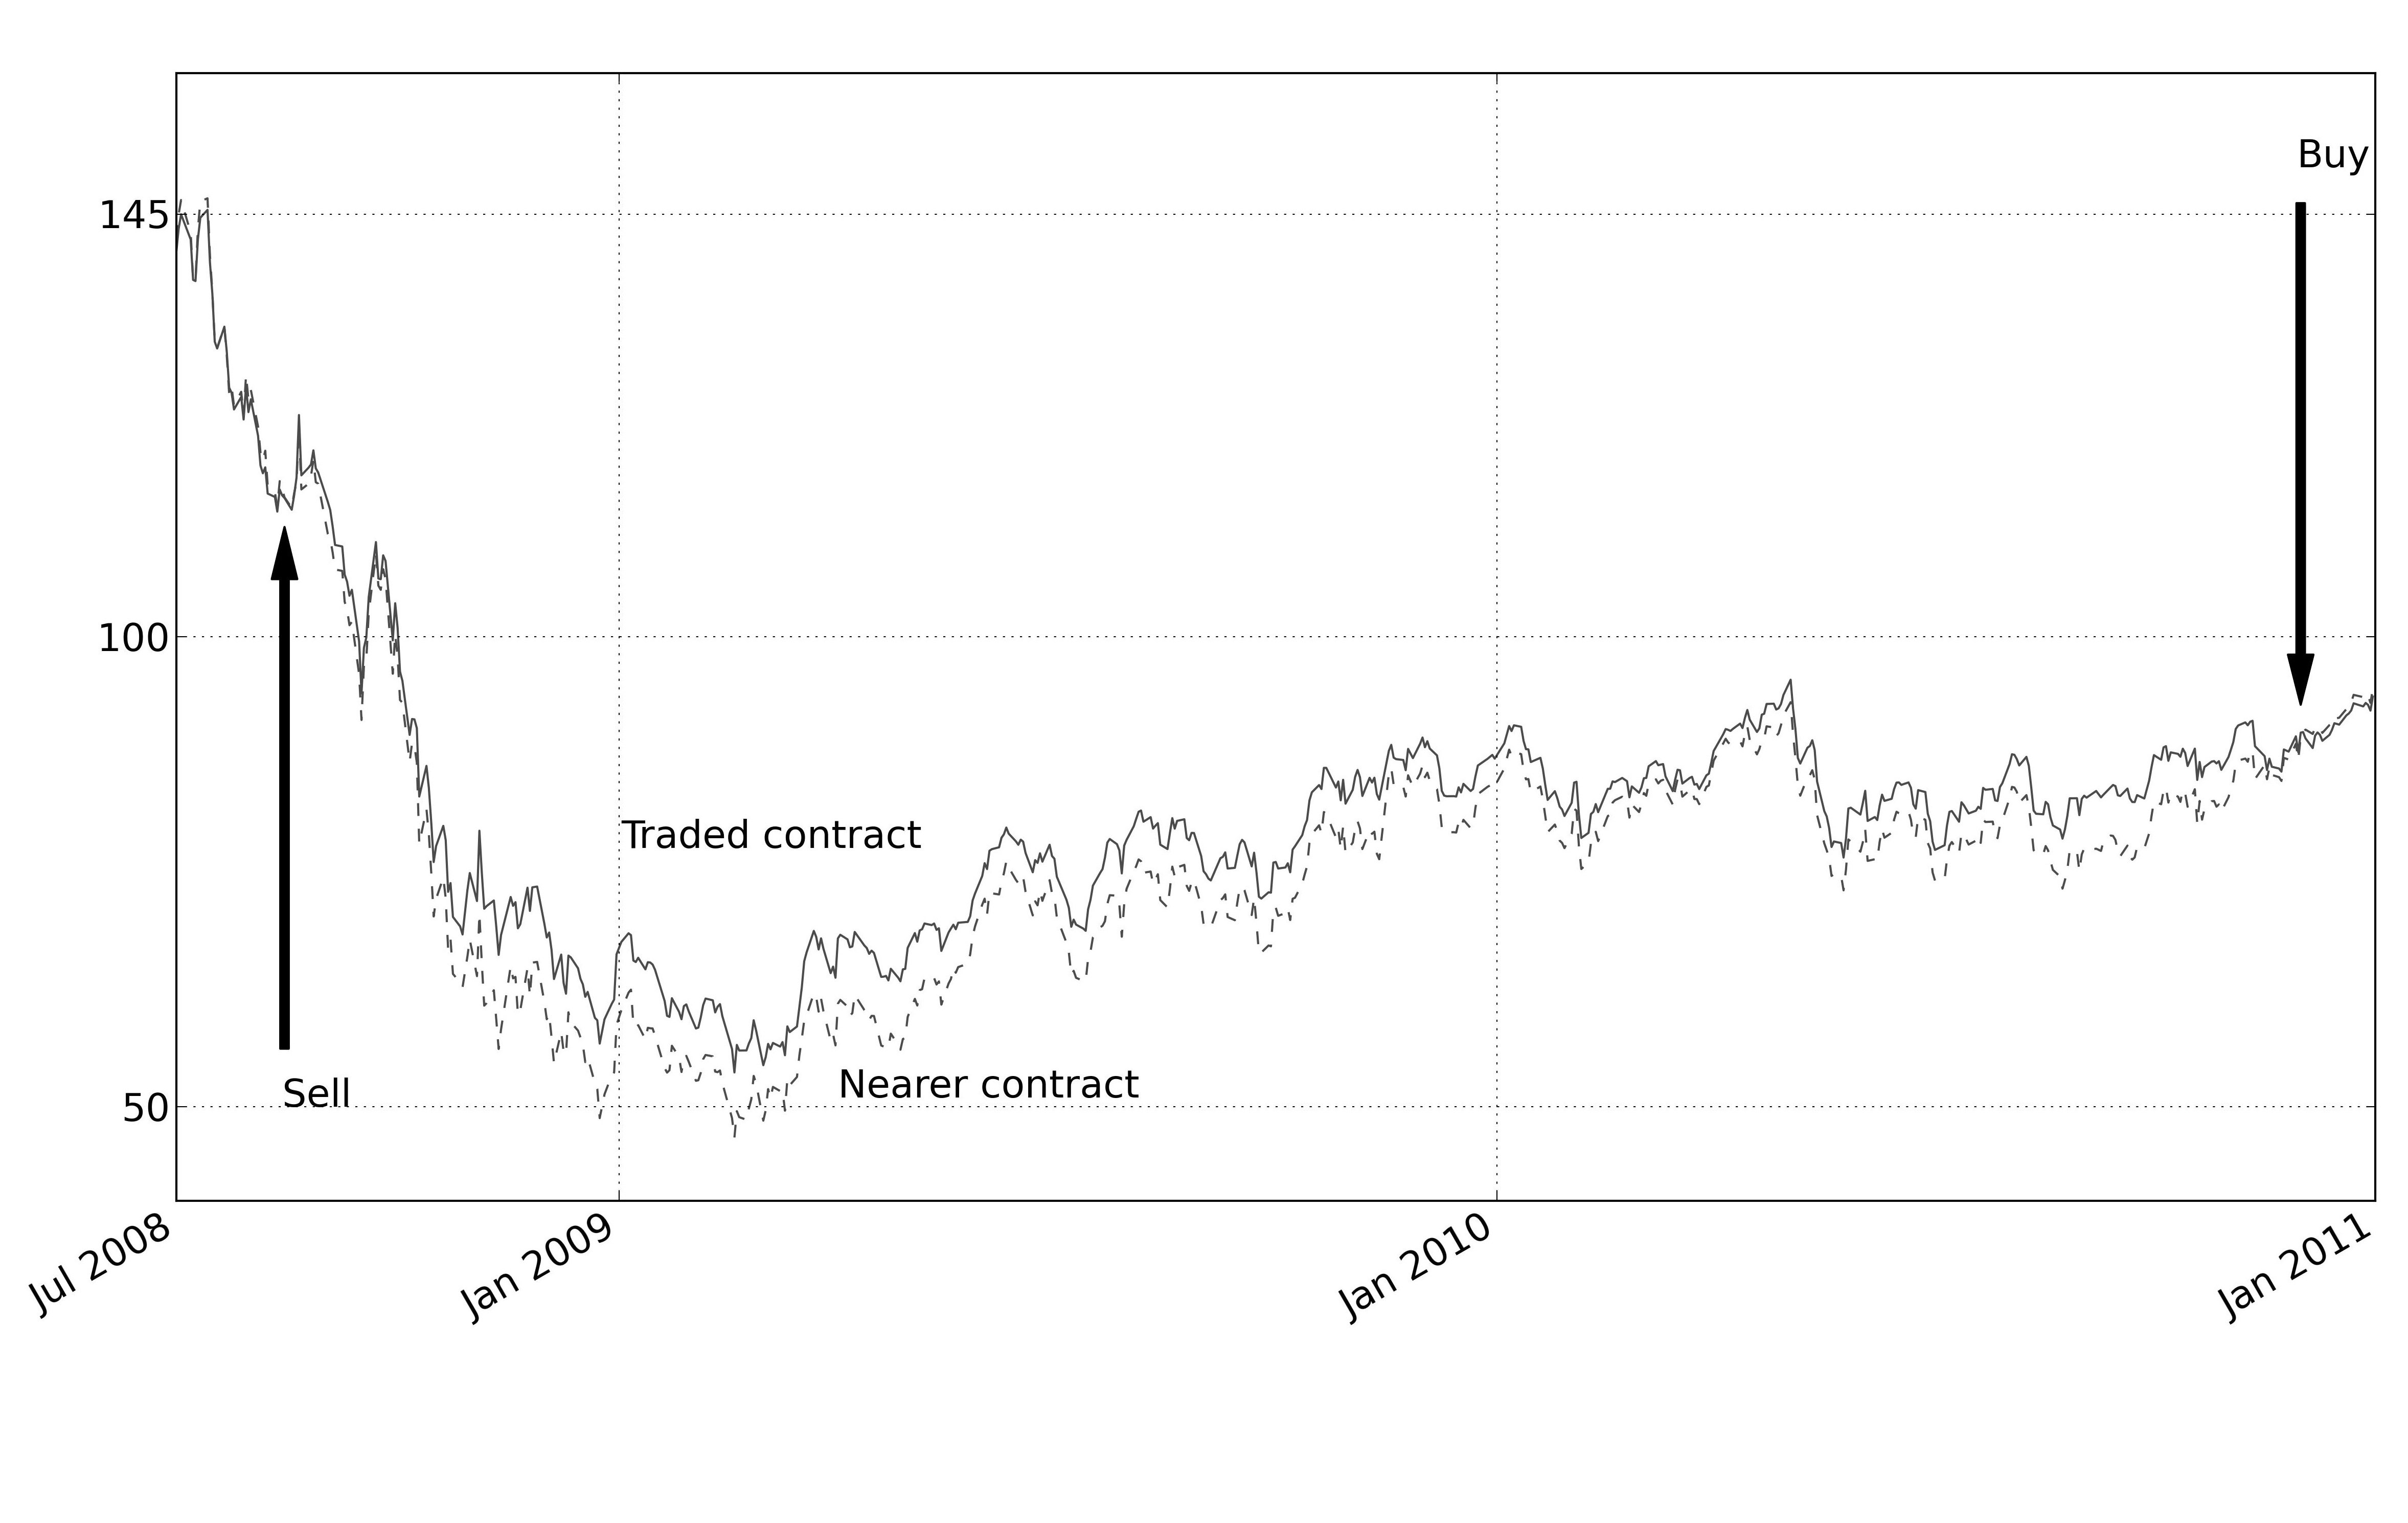
\includegraphics[width=\textwidth]{figures/raw/img-019.png} \caption{TRADING CRUDE OIL WITH CARRY IN 2008-10. WE ARE SLOW TO SELL AND STAY SHORT TOO LONG\\
使用 Carry 规则交易 2008 至 2010 年的原油。我们卖出动作偏慢，而且空头持有得过久}\end{figure}

\begin{englishblock} Unfortunately it remains bearish long after the market has turned, but you can't win them all. It makes sense to combine diversifying trading rules like the positive skew, trend following EWMAC rule, with a negative skew carry rule. \end{englishblock}

\begin{chineseblock}遗憾的是，即便市场已经转向，它仍然会长时间保持看空。但你不可能事事都赢。因此，把像 EWMAC 这样具有正偏度的趋势跟踪规则，与 carry 这种负偏度规则组合起来，从分散化角度看是很有意义的。\end{chineseblock}

\bilingualsection{Adapting and creating trading rules}{改造并创建交易规则}

\bilingualsubsection{Staunch Systems Trader}{坚定的系统化交易者}

\begin{englishblock} The above trading rules, one positive and one negative skew, are sufficient to create a pretty good trading strategy. The benefits of adding further rules within the same styles are relatively limited. Just using these two simple rules would generate roughly 85\% of the back-tested performance of my own more complicated system. However you might still want to create your own rules, or adapt those you find elsewhere. Here are some pointers, with an example of how I modified a trading rule I read about whilst researching this chapter, which I've nicknamed ‘Close to Open'. Simplicity and Trading rules in books tend to be quite complicated, with lots of objectivity conditionals and a degree of subjectivity. Try and pare the rule down to its essential elements, to create a simple and objective trading rule. The example rule I found could be reduced to ‘Buy if the open is higher than yesterday's close'. (I haven't tested this rule and I have no idea if it will work or not.) Continuous, Many trading rules are unfortunately of a buy or sell, binary, nature. If not binary possible you should make them continuous. I converted the simple rule above to calculate the raw forecast as [Open price - Close price]. Not market The value of a forecast should be comparable across markets and across specific; time. If a forecast is in price units, as in the simple example here, then you volatility should volatility standardise it to get a forecast proportional to Sharpe standardised ratio. So your forecast would be: [Open price - Close price ] ÷ (Recent standard deviation of daily returns) This is the same standardisation that I use in the EWMAC and Carry rules. Changing Separate entry and exit rules are not suitable for the framework.* Ideally a forecast forecast should change continuously, independently of what our position is, throughout the life of a trade. This suggests that you should create rules which recalculate forecasts every time you have new data, and then adjust your positions accordingly. Normally this is simply a matter of modifying the entry rule. Rather than use the ‘Close to Open' rule only for entries, you would calculate the forecast value every day. Correct scaling If you're going to create trading rules you need to rescale them from their natural scaling, so that the expected absolute value of the forecast is around 10. You do this by multiplying your raw forecast by a forecast scalar. You need to back-test the behaviour of the rule with real data to find the average forecast, but in line with my recommendations in chapter three, ‘Fitting', you shouldn't look at performance data whilst doing this. See appendix D, page 297, for more details. The natural average absolute value of this rule is 0.33, implying the forecast scalar in this case is 10 ÷ 0.33 = 30. * If you absolutely have to use an entry rule which doesn't adjust throughout the life of the trade, with a separate exit rule, then I strongly suggest you use the stop loss rule I advocate for semi-automatic traders. I don't recommend using any other kind of explicit exit rule as they are usually over-fitted and make life very complicated. \end{englishblock}

\begin{chineseblock}上面介绍的两条交易规则，一条正偏度、一条负偏度，已经足够构建出一套相当不错的交易策略了。在相同风格下继续加入更多规则，带来的边际收益其实相对有限。光是使用这两条简单规则，就能达到我自己那套更复杂系统大约 85\% 的回测表现。不过，你也许仍然想设计自己的规则，或者改造你在别处看到的规则。下面是一些建议，同时我也会给出一个例子，说明我在研究本章时读到一条交易规则后，是如何把它修改成我称之为“Close to Open”的规则的。简洁性与客观性 书里的交易规则往往写得很复杂，夹杂大量条件判断，并且多少带有一些主观性。你应该尽量把规则削减到只剩最核心的要素，从而得到一条简单而客观的交易规则。比如我看到的那个例子，最终就可以被简化为：“如果今天开盘价高于昨天收盘价，就买入。”（我并没有测试过这条规则，所以我也不知道它到底有没有用。）连续性，而非二元 很多交易规则不幸天生就是二元的，只能给出“买”或“卖”。如果可能的话，你应当尽量把它们改造成连续型规则。我就把上面那条简单规则改造成了一个原始预测值，写成 [开盘价 - 收盘价]。不要依赖特定市场；要做波动率标准化 预测值的数值，应当在不同市场之间、也应当在不同时间之间具备可比性。如果一个预测值是以价格单位表示的，就像这个例子一样，那么你就应当把它做波动率标准化，使其变成与夏普比率成正比的预测值。因此，你的预测值应当写成：[开盘价 - 收盘价] ÷（近期日收益标准差）。这和我在 EWMAC 与 Carry 规则中所使用的标准化方法是相同的。预测值必须持续变化 框架并不适合那种把入场规则和离场规则完全分开的做法。理想情况下，预测值应当在整笔交易的生命周期里持续变化，并且这种变化应当独立于当前仓位。这意味着，你设计的规则应当能够在每次获得新数据时重新计算预测值，然后相应调整仓位。通常，这只是修改入场规则的问题。与其让“Close to Open”规则只在入场时发挥作用，不如每天都去重新计算它的预测值。正确缩放 如果你准备创建交易规则，就必须把它们从原生尺度上重新缩放，使得预测值的预期平均绝对值大约为 10。做法是把原始预测值乘上一个预测缩放因子（forecast scalar）。你需要用真实数据回测这条规则的行为，以找出平均预测值；但按照我在第三章“拟合”中的建议，在做这件事时你不应查看表现数据。更多细节见附录 D，第 297 页。这条规则的自然平均绝对值是 0.33，因此它的预测缩放因子就是 10 ÷ 0.33 = 30。* 如果你无论如何都必须使用那种在整笔交易生命周期中不会持续更新的入场规则、并另配独立离场规则，那么我强烈建议你使用我为半自动交易者推荐的止损规则。我不建议使用其他任何显式离场规则，因为它们通常都过拟合，而且会让整个系统变得异常复杂。\end{chineseblock}

\bilingualsection{Selecting trading rules and variations}{选择交易规则与变体}

\bilingualsubsection{Staunch Systems Trader}{坚定的系统化交易者}

\begin{englishblock} Even if you don't adapt or create new rules and just use mine, there are still a theoretically infinite number of EWMAC trading rule variations on the menu. If you do get creative and make your own rules the number of options will explode. Which rules and variations should you use in practice? As I said in chapter three, ‘Fitting', I don't recommend using back-tested profitability to select trading rules or variations. Instead you should focus on behaviour such as the correlation between variations, and the speed they trade at, whilst ignoring Sharpe ratio and other performance metrics. You should then use two selection criteria. The first is to avoid including any two variations with more than a 95\% correlation to each other, as one of them will not be adding any value to the system. I discuss how to prune possible variations of the EWMAC rule in appendix B (in the section on EWMAC, from page 282). Secondly, you must exclude anything which trades too slowly, or too quickly. As I mentioned in chapter two, very slow rules are unlikely to generate significant Sharpe ratio.85 I suggest you remove any rule which holds positions for longer than a few months. At the other end of the spectrum for many instruments fast rules will be too expensive to trade. This could mean you end up choosing a different set of variations for each instrument. I'll return to this in chapter twelve, ‘Speed and Size', where I'll show how to determine which variations should be excluded for a given level of trading costs. The staunch systems trader example chapter in part four will give an overview of the rule selection process. \end{englishblock}

\begin{chineseblock}即便你不去改造或创造新规则，而只是照用我的规则，理论上 EWMAC 这条规则本身也依然有无限多种变体可供选择。如果你开始发挥创造力、自己设计规则，可选项的数量就更会爆炸式增加。那么，实际中你到底该用哪些规则和哪些变体？正如我在第三章“拟合”中说过的，我不建议你根据回测盈利能力去选择交易规则或变体。相反，你应当关注的是这些规则的行为特征，例如不同变体之间的相关性，以及它们交易的速度，而忽略夏普比率及其他表现指标。之后，你应该使用两条筛选标准。第一，不要把任何两个彼此相关性超过 95\% 的变体同时放进系统，因为其中一个不会再给系统增加任何额外价值。我在附录 B （EWMAC 部分，第 282 页起）中讨论了，如何修剪 EWMAC 规则的可能变体。第二，你必须剔除那些交易得过慢或过快的规则。正如我在第二章中提到的，交易特别慢的规则不太可能产生显著的夏普比率。85 我建议你去掉任何平均持仓时间长于几个月的规则。而在光谱的另一端，对于许多品种而言，交易过快的规则则会因为成本过高而不适合使用。这意味着，你最终可能不得不为不同品种选择不同的规则变体集合。我会在第十二章“速度与规模”中回到这一点，并说明在既定交易成本水平下，如何判断哪些变体应当被排除。第四部分里“坚定的系统化交易者”那个示例章节，也会给出这一规则筛选流程的整体概览。\end{chineseblock}

\bilingualsection{Summary of trading rules and forecasts}{交易规则与预测值总结}

\begin{englishblock} Where do If you're staunch systems traders then each of your trading rules forecasts come produces a forecast, including any variations that we're using; for from example to capture different trend lengths. Asset allocating investors use a constant identical forecast for all instruments. Semi-automatic traders make discretionary forecasts on an ad-hoc basis for a changing set of instruments. \end{englishblock}

\begin{chineseblock}预测值从哪里来？ 如果你是坚定的系统化交易者，那么你的每一条交易规则都会生成一个预测值，其中也包括你所使用的各种规则变体--- 比如用来捕捉不同趋势长度的那些变体。资产配置型投资者则对所有品种使用一个恒定且相同的预测值。半自动交易者则针对一个不断变化的品种集合，临时性地给出主观预测。\end{chineseblock}

\bipairgap

\begin{englishblock} Forecast for every For staunch systems traders each instrument will have a separate instrument and forecast for a given trading rule variation. So if you had ten instruments from each trading and three different kinds of trading rule, each with two variations, then rule you'd calculate 10 × 3 × 2 = 60 individual forecasts. Semi-automatic traders and asset allocating investors have one forecast per instrument. \end{englishblock}

\begin{chineseblock}每个品种、每条规则都要有预测值 对坚定系统化交易者来说，每个品种在每个交易规则变体下都应当有一个单独预测值。因此，如果你有 10 个品种、3 类不同交易规则，而每类规则又各有 2 个变体，那么你就需要计算 10 × 3 × 2 = 60 个单独预测值。半自动交易者和资产配置型投资者则是每个品种只有一个预测值。\end{chineseblock}

\bipairgap

\begin{englishblock} Forecast sign is Positive means you buy and go long the asset. A negative forecast vital means you go short. A zero forecast means you shouldn't have a position. \end{englishblock}

\begin{chineseblock}预测值的正负至关重要 正值意味着你买入并做多该资产。负预测值意味着你做空。零预测值意味着你不应持有仓位。\end{chineseblock}

\bipairgap

\begin{englishblock} Forecast size is Absolutely larger forecasts mean you are more confident of your also important opinion and expect a bigger rise (or fall) in prices. Forecasts should have an expected absolute value of 10. \end{englishblock}

\begin{chineseblock}预测值大小同样重要 预测值绝对值越大，意味着你对自己的判断越有信心，也预期价格会出现更大的上涨（或下跌）。预测值的预期绝对值平均应为 10。 \end{chineseblock}

\bipairgap

\begin{englishblock} Forecasts Forecasts must lie in the range -20 to +20, unless you can't short an shouldn't be too instrument in which case it would be between 0 and +20. If a trading big rule produces a larger forecast then cap it at either end of the range. \end{englishblock}

\begin{chineseblock}预测值不应过大 预测值必须位于 -20 到 +20 之间；如果你无法做空某个品种，那么区间就应为 0 到 +20。如果某条交易规则生成了更大的预测值，就应当把它封顶到区间边界。\end{chineseblock}

\bipairgap

\begin{englishblock} Semi-automatic Make your own predictions and convert them into forecasts between traders: -20 (strongly bearish) and +20 (strongly bullish). Positions are closed using systematic stop loss rule, as described in chapter thirteen. \end{englishblock}

\begin{chineseblock}半自动交易者： 自己做出判断，并把它转换成 -20（极度看空）到 +20（极度看多）之间的预测值。头寸则通过系统化止损规则来关闭，详见第十三章。\end{chineseblock}

\bipairgap

\begin{englishblock} Asset allocating Use a constant forecast of +10 for all assets. investors: \end{englishblock}

\begin{chineseblock}资产配置型投资者： 对所有资产使用恒定的 +10 预测值。\end{chineseblock}

\bipairgap

\begin{englishblock} Staunch Use a combination of systematic trading rules like EWMAC and Carry, systematic design your own rule or adapt others. Follow the advice earlier in this traders: chapter, and in chapter three, when selecting trading rule variations. \end{englishblock}

\begin{chineseblock}坚定的系统化交易者： 使用像 EWMAC 和 Carry 这样的系统化交易规则组合，或者自己设计规则、改造他人的规则。在选择交易规则变体时，请遵循本章以及第三章中给出的建议。\end{chineseblock}

\bipairgap

\begin{englishblock} You should now have one, or more, trading rules ready to go. Asset allocating investors will be using the single ‘no rule' rule, and semi-automatic traders will be making discretionary forecasts. If you're in either of these groups you can skip to chapter nine. Semi-automatic traders should either have developed their own rules, adapted a publically available rule, or be happy for now to use one or both of the rules I provided earlier in the chapter. If you have only one trading rule variation you can also skip the next chapter. But if you're using multiple rules or variations then you'll need to read chapter eight to discover how to combine forecasts from different rules. \end{englishblock}

\begin{chineseblock}到现在，你应该已经准备好一条或多条可以直接投入使用的交易规则了。资产配置型投资者会使用那条单一的“无规则”规则，而半自动交易者则会给出主观预测。如果你属于这两类人中的任意一种，现在就可以直接跳到第九章。半自动交易者应当已经建立起自己的规则，或者改造了某条公开可见的规则；又或者至少暂时愿意使用我在本章前面提供的一条或两条规则。如果你只使用一个交易规则变体，那么你也可以跳过下一章。但如果你打算使用多条规则或多个变体，那么你就需要阅读第八章，以了解如何把来自不同规则的预测值组合起来。\end{chineseblock}
